\chapter{Vektorb"undel}

Betrachte $\T M$ als glatte Mannigfaltigkeit durch
	\[ \begin{array}{ccc} \T M|_U = \pi^{-1}(U) &\to& \varphi(U) \times \R^m \cong U \times \R^m \\
		X_p = \sum \xi^i\pdifffrac[p]{}{x^i} &\mapsto& \left(\varphi(p),\xi\right). \end{array} \]
Fasern : $\T_pM = \pi^{-1}(p)$ $m$-dimensionaler Vektorraum und $X_p = \sum \xi^i \pdifffrac[p]{}{x^i} \mapsto \xi$ ist ein linearer Isomorphismus.

% Definition 5.1
\begin{Dfn}
  Ein \CmMark[Vektorb{\"u}ndel!glattes reelles]{glattes reelles Vektorb"undel} vom Rang $k$ "uber einer glatten Mannigfaltigkeit $M$ ist eine glatte Mannigfaltigkeit $E$, der sogenannte \CmMark{Totalraum} des B"undels, zusammen mit einer glatten Abbildung $\pi \colon E \to M$, der Projektion, sodass f"ur jedes $p \in M$ gilt:
  \begin{enumerate}[label=(\roman*)]
  \item Die Faser $E_p = \pi^{-1}(p)$ trägt die Struktur eines $k$-dimensionalen reellen Vektorraumes.
  \item Es existiert eine Umgebung $U$ von $p$ in $M$ und ein Diffeomorphismus
    \begin{align*}
      \tau \colon E|_U = \pi^{-1}(U) \to U \times \R^k,
    \end{align*}
    so dass die Einschränkung
    \begin{align*}
      \tau_p \colon E_p \to \R^k \quad ( \cong \{p\} \times \R^k)
    \end{align*}
    ein linearer Isomorphismus ist.
    Ein solches $\tau$ heißt \CmMark{B"undelkarte}.
  \end{enumerate}
\end{Dfn}

\begin{bsp}
  \begin{enumerate}[label=(\arabic*)]
  \item $E = M \times \R^k$ mit $\pi \colon E \to M, (p,x) \mapsto p$.
  \item Das Tangentialb"undel $\T M$ auf $M$.
  \item Ist $E \xrightarrow{\pi} M$ ein Vektorb"undel "uber $M$ und $U \subseteq M$ offen (oder eine Untermannigfaltigkeit), so ist $E|_U = \pi^{-1}(U)$ ein Vektorb"undel "uber $U$.
  \end{enumerate}
\end{bsp}

Ein \CmMark{Vektorb"undelmorphismus} zwischen zwei Vektorb"undeln $E \xrightarrow{\pi} M$ und $E' \xrightarrow{\pi'} N$ ist eine glatte Abbildung $F \colon E \to E'$, so dass eine glatte Abbildung $f$ existiert f"ur die das folgende Diagram kommutiert

\begin{center}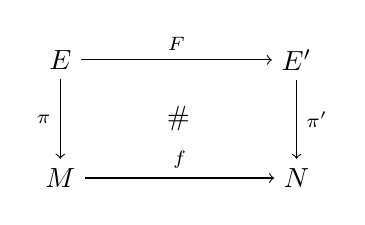
\begin{tikzpicture}
	%\draw[step=0.25,gray!15] (-6,-1) grid (6,5); \draw[step=0.5,gray!30] (-6,-1) grid (6,5); \fill (0,0) circle(0.1); %Hilfsgitter
	\node (E) at (-1.5,0.75) {$E$}; \node (E') at (1.5,0.75) {$E'$}; \node (M) at (-1.5,-0.75) {$M$}; \node (N) at (1.5,-0.75) {$N$};
	
	\draw[->] (E) --node[above,font=\scriptsize]{$F$} (E'); \draw[->] (M) --node[above,font=\scriptsize]{$f$} (N);
	\draw[->] (E) --node[left,font=\scriptsize]{$\pi$} (M); \draw[->] (E') --node[right,font=\scriptsize]{$\pi'$} (N);
	
	\node at (0,0) {$\#$};
\end{tikzpicture}\end{center}

und ferner f"ur $p \in M$ die Abbildung $E_p \xrightarrow{F} E'_{f(p)}$ linear ist.

Gilt $M = N$ so ist ein $M$-Vektorb"undelmorphismus $F$ von $E$ nach $E'$ eine glatte Abbbildung $F \colon E \to E'$, so dass das folgende Diagram kommutiert und $F$ faserweise linear ist.

\begin{center}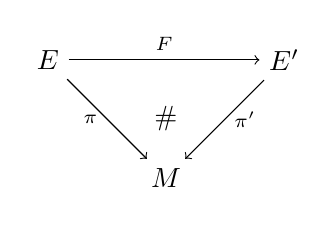
\begin{tikzpicture}
	%\draw[step=0.25,gray!15] (-6,-1) grid (6,5); \draw[step=0.5,gray!30] (-6,-1) grid (6,5); \fill (0,0) circle(0.1); %Hilfsgitter
	\node (E) at (-1.5,0.75) {$E$}; \node (E') at (1.5,0.75) {$E'$}; \node (M) at (0,-0.75) {$M$};
	
	\draw[->] (E) --node[above,font=\scriptsize]{$F$} (E');
	\draw[->] (E) --node[left,font=\scriptsize]{$\pi$} (M); \draw[->] (E') --node[right,font=\scriptsize]{$\pi'$} (M);
	
	\node at (0,0) {$\#$};
\end{tikzpicture}\end{center}

Die Vektorb"undel $E,E'$ "uber $M$ heißen \CmMark[Vektorb{\"u}ndel!isomorphes]{isomorph}, wenn ein $M$-Vektor"-b"undel"-morphismus
$G$ existiert mit $G F = \Id_E$ und $FG = \Id_{E'}$.
Dies ist genau dann der Fall, wenn $F$ faserweise ein Inverses besitzt.
(Der Beweis dieser Aussage sei als "Ubungsaufgabe "uberlassen.)

Ein Vektorb"undel $E \xrightarrow{\pi} M$ heißt \CmMark[Vektorb{\"u}ndel!triviales]{trivial}, wenn es einen Vektorb"undelisomorphismus von $E$ auf $M \times \R^k$ gibt. Jedes
\begin{align*}
  \tau \colon E|_U \to U \times \R^k
\end{align*}
ist ein Vektorb"undelisomorphismus.
Die B"undelkarten werden daher auch \CmMark[Trivialisierung!lokale]{lokale Trivialisierungen} genannt.

Es sei $(\tau_\alpha,U_{\alpha})_{\alpha \in \calI}$ eine Familie lokaler Trivialisierungen von $E$ mit $M = \bigcup_{\alpha \in J}U_{\alpha}$.
Der Diffeomorphismus
\begin{align*}
  \tau_{\alpha} \circ \tau_{\beta}^{-1}\colon (U_{\alpha} \cap U_{\beta}) \times \R^k \to (U_{\alpha} \cap U_{\beta}) \times \R^k
\end{align*}
definiert die sogenannten \CmMark{{\"U}bergangsfunktionen}
\begin{align*}
  g_{\alpha\beta} \colon U_{\alpha} \cap U_{\beta} \to \gls{GL}_k(\R)
\end{align*}
durch 
\begin{align*}
  \tau_{\alpha} \circ \tau_{\beta}^{-1}(p,x) = (p,g_{\alpha\beta}(p) x).
\end{align*}
Die "ubergangsfunktionen sind glatt und f"ur alle $p \in U_{\alpha} \cap U_{\beta} \cap U_{\gamma}$ gilt:
\begin{align*}
  g_{\alpha\gamma}(p) = g_{\alpha\beta}(p) \cdot g_{\beta\gamma}(p),
\end{align*}
denn
\begin{align*}
	(p,g_{\alpha\gamma}(p)x) & = \tau_{\alpha} \circ \tau_{\gamma}^{-1}(p,x)\\
	& = \tau_{\alpha} \circ \tau_{\beta}^{-1} \circ \tau_{\beta} \circ \tau_{\gamma}^{-1}(p,x)\\
	& = (\tau_{\alpha} \circ \tau_{\beta}^{-1})(p,g_{\beta\gamma}(p)x)\\
	& = (p,g_{\alpha\beta}(p)\cdot g_{\beta\gamma}(p)x).
\end{align*}

\begin{bsp}
  Die "ubergangsfunktionen von $\T M$ sind gegeben durch
  \begin{align*}
    \D(\psi \circ \varphi^{-1}) = \left(\partial_i(\psi^j \circ \varphi^{-1})\right)_{i,j \leq m}.
  \end{align*}
\end{bsp}

% Satz 5.2
\begin{Satz}\label{satz-5-2}
  Es sei $M$ eine glatte Mannigfaltigkeit mit einer offenen "Uberdeckung $\{U_{\alpha}\}_{\alpha \in \calI}$ und einer glatten Abbildung
  \begin{align*}
    g_{\alpha\beta} \colon U_{\alpha} \cap U_{\beta} \to \Gl_k(\R)
  \end{align*}
so dass f"ur alle $\alpha,\beta,\gamma \in \calI$ und $p \in U_{\alpha} \cap U_{\beta} \cap U_{\gamma}$ gilt:
\begin{align*}
  g_{\alpha\gamma} (p) = g_{\alpha\beta}(p)g_{\beta\gamma}(p).
\end{align*}
Dann ist
	\[ E = \bigcup_{\alpha \in \calI}^{\cdot} \FakRaum{U_{\alpha} \times \R^k}{\sim}, \]
wobei $(p,x)_{\alpha} \sim (q,y)_{\beta}$ genau dann gilt, wenn $p = q$ und $x = g_{\alpha\beta}(p)y$, ein glattes Vektorb"undel.
\end{Satz}

Der Beweis sei erneut als Aufgabe "uberlassen.

\begin{kor}
  Ist $E$ ein glattes Vektorb"undel "uber $M$ mit "Ubergangsfunktionen $\{g_{\alpha\beta}\}$, so ist das oben konstruierte Vektorb"undel isomorph zu $E$.
\end{kor}

Es sei $E \xrightarrow{\pi} N$ ein Vektorb"undel und $\Phi \colon M \to N$ glatt.
Das längs $\Phi$ zur"uckgezogene B"undel ("`\CmMark{pullback}"') ist definiert durch den Totalraum
\begin{align*}
  E' = \Phi^{\ast}E = \{(p,x) \mid x \in E_{\Phi(p)}\} \subseteq M \times E,
\end{align*}
die Projektion $\pi' \colon \Phi^{\ast}E \to M, (p,x) \mapsto p$ und die folgenden B"undelkarten:
Es sei $p \in M$ und $(\tau, U)$ eine B"undelkarte von $E$ um $\Phi(p)$, sowie $(\varphi,V)$ eine Karte von $M$ um $p$ mit $\Phi(V) \subseteq U$.
Dann definiert 
\begin{align*}
  \Phi^{\ast}E|_V \to V \times \R^k, (p,x) \mapsto \left(p, \tau_{\Phi(p)}(x)\right)
\end{align*}
eine B"undelkarte.

Sind $E \xrightarrow{\pi} M, E' \xrightarrow{\pi'} N$ Vektorb"undel, dann ist $E \times E' \xrightarrow{\pi \times \pi'} M \times N$ mit lokalen Trivialisierungen $\tau \times \tau'$ ebenfalls ein Vektorb"undel.
Insbesondere ist im Falle $M = N$ $E \times E'$ ein B"undel "uber $M \X M$.
Es sei $\Delta \colon M \to M \times M$, $p \mapsto (p,p)$.

\begin{center}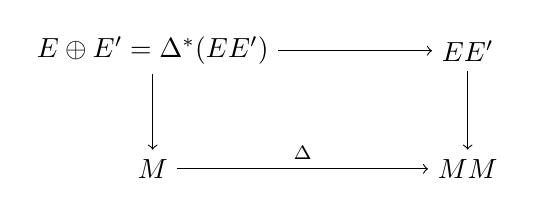
\begin{tikzpicture}
	%\draw[step=0.25,gray!15] (-6,-1) grid (6,5); \draw[step=0.5,gray!30] (-6,-1) grid (6,5); \fill (0,0) circle(0.1); %Hilfsgitter
	\node (1) at (-2,0.75) {$E \oplus E' = \Delta^*(E \X E')$}; \node (2) at (2,0.75) {$E \X E'$}; \node (3) at (-2,-0.75) {$M$}; \node (4) at (2,-0.75) {$M \X M$};
	
	\draw[->] (1) -- (2); \draw[->] (3) --node[above,font=\scriptsize]{$\Delta$} (4);
	\draw[->] (1) -- (3); \draw[->] (2) -- (4);
\end{tikzpicture}\end{center}

Das längs $\Delta$ zur"uckgezogene B"undel $E \oplus E' = \Delta^{\ast}(E \times E')$ heißt die \CmMark{Whitneysumme} von $E$ und $E'$.
Faserweise gilt
\begin{align*}
  (E \oplus E')_p = E_p \oplus E'_p.
\end{align*}
 
\emph{"Uberlege:} $\Hom(E,E')$, sowie $E \otimes E', \bigotimes E$ und $\Lambda^pE, \Lambda E$ sind "`vern"unftige"' B"undel.

\section{Intermezzo: Multilineare Algebra}
Es seien $V$ und $W$ $k$-Vektorr"aume. Das \CmMark{Tensorprodukt} $V \otimes W$ ist der von den Elementen $v \otimes w$ mit $v \in V$, $w \in W$ und den Relationen \begin{enumerate}[label=(\roman*),widest=iii]
\item
	$(v + v') \otimes w = v \otimes w + v' \otimes w$
\item
	$v \otimes (w + w') = v \otimes w + v' \times w'$
\item
	$(\lambda v) \otimes w = \lambda (v \otimes w) = v \otimes (\lambda w)$
\end{enumerate} erzeugte Vektorraum.

\begin{emptythm}[Eigenschaften:]\begin{enumerate}[label=\arabic*),leftmargin=*]
\item
	Die Abbildung $b: V \X W \to V \otimes W$, $(v, w) \mapsto v \otimes w$ ist bilinear.
\item
	$v \otimes w = 0 \Leftrightarrow v = 0$ oder $w = 0$
\item
	$V \otimes k \cong V$
\item
	$V \otimes W \cong W \otimes V$
\item
	$V^* \otimes W \cong \Hom(V, W)$ verm"oge $(\varphi \otimes w)(v) = \varphi(v) \cdot w$ wobei $V^*$ der \gls{Dualraum} zu $V$ ist
\item
	Sind $\{v_i\}_{i \in \calI}$ und $\{w_j\}_{j \in \calJ}$ Basen von $V$ und $W$, so ist $\{v_i \otimes w_j\}_{(i,j) \in \calI \X \calJ}$ eine Basis von $V \otimes W$. Insbesondere gilt f"ur Vektorr"aume endlicher Dimension dass $\ddim (V \otimes W) = \ddim V \cdot \ddim W$
\end{enumerate}\end{emptythm}

\begin{emptythm}[Universelle Eigenschaft:]
Ist $U$ ein Vektorraum und $\beta$ eine bilineare Abbildung von $V \X W$ in $U$. Dann existiert genau eine lineare Abbildung $\varphi: V \otimes W \to U$ mit $\beta = \varphi \circ b$.
\begin{center}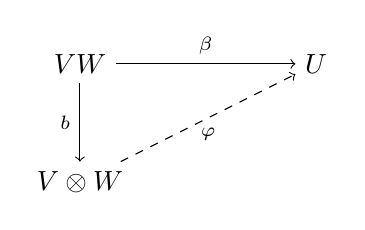
\begin{tikzpicture}
	\node (1) at (-2,0) {$V \X W$}; \node (2) at (1,0) {$U$}; \node (3) at (-2,-1.5) {$V \otimes W$};
	\draw[->] (1) --node[above,font=\scriptsize]{$\beta$} (2);
	\draw[->] (1) --node[left,font=\scriptsize] {$b$} (3);
	\draw[->,dashed] (3) --node[below,font=\scriptsize] {$\varphi$} (2);
\end{tikzpicture}\end{center}
Diese Eigenschaft bestimmt $(V \otimes W, b)$ eindeutig bis auf Isomorphie.
\end{emptythm}

Das Bilden von Tensorprodukten ist bis auf Isomorphie assoziativ. Man schreibt daher
	\[ \bigotimes^p V = \underbrace{V \otimes \ldots \otimes V}_{p\text{-mal}} \]
Setzt man $\bigotimes^0 V = k$, so wird $\bigotimes V = \bigoplus_{p=0}^{\infty} \bigotimes^p V$ mit dem durch die Zuordnungen
	\[ (v_1 \otimes \ldots \otimes v_{p+1} \otimes \ldots \otimes v_{p+q}) \mapsto v_1 \otimes \ldots \otimes v_{p+q} \in \bigotimes^{p+q} V \]
induzierten Produkt zu einer graduierten Algebra.

Das $p$-fach \CmMark[Produkt!{\"a}u{\ss}eres]{"au"sere Produkt} $\Lambda^pV$ ist der von den Elementen $v_1 \wedge \ldots \wedge v_p$, $v_i \in V$ und den Relationen \begin{enumerate}[label=(\roman*),widest=iii]
\item
	$v_1 \wedge \ldots \wedge v_i \wedge v_{i+1} \wedge \ldots \wedge v_p = - v_1 \wedge \ldots \wedge v_{i+1} \wedge v_i \wedge \ldots \wedge v_p$ (Schiefsymmetrie)
\item
	$(v_1 + w_1) \wedge \ldots \wedge v_p = v_1 \wedge \ldots \wedge v_p + w_1 \wedge v_2 \wedge \ldots \wedge v_p$
\item
	$(\lambda v_1) \wedge \ldots \wedge v_p = \lambda (v_1 \wedge \ldots \wedge v_p)$
\end{enumerate}
erzeugte Vektorraum.

\begin{emptythm}[Eigenschaften:]\begin{enumerate}[label=\arabic*),leftmargin=*]
\item
	Die Abbildung $s: V \X \ldots \X V \to \Lambda^p V$, $(v_1,\ldots ,v_p) \mapsto v_1 \wedge \ldots \wedge v_p$ ist multilinear und schief
\item
	Es gilt $v_1 \wedge \ldots \wedge v_p = 0$ genau dann wenn $v_1, \ldots , v_p$ linear abh"angig sind
\item
	Ist $\{e_i\}_{i \le n}$ eine Basis von $V$, so ist $\{e_{i_1} \wedge \ldots \wedge e_{i_p} | i_1 < i_2 < \ldots < i_p\}$ eine Basis von $\Lambda^pV$, es gilt also $\ddim \Lambda^pV = \left( \begin{smallmatrix} n \\ p \end{smallmatrix} \right)$. Insbesondere ist $\Lambda^pV = 0$ falls $p > n$ und $\ddim \Lambda^nV = 1$ und f"ur $v_i = \sum \alpha_i^j e_j$ gilt:
		\[ v_1 \wedge \ldots \wedge v_p = \ddet (\alpha_i^j) \cdot e_1 \wedge \ldots \wedge e_n \]
\end{enumerate}\end{emptythm}

\begin{emptythm}[Universelle Eigenschaft:]
Ist $U$ ein Vektorraum und $\sigma$ eine schiefsymmetrische multilineare Abbildung $\underbrace{V \X \ldots  \X V}_{p\text{-mal}} \to U$, so existiert genau eine lineare Abbildung $\varphi: \Lambda^pV \to U$ mit $\sigma = \varphi \circ s$.
\begin{center}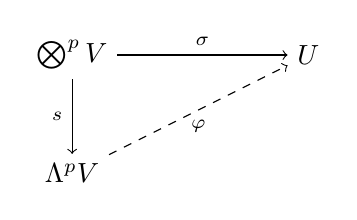
\begin{tikzpicture}
	\node (1) at (-2,0) {$\bigotimes^pV$}; \node (2) at (1,0) {$U$}; \node (3) at (-2,-1.5) {$\Lambda^pV$};
	\draw[->] (1) --node[above,font=\scriptsize]{$\sigma$} (2);
	\draw[->] (1) --node[left,font=\scriptsize] {$s$} (3);
	\draw[->,dashed] (3) --node[below,font=\scriptsize] {$\varphi$} (2);
\end{tikzpicture}\end{center}
Die Isomorphieklasse von $(\Lambda^pV, s)$ ist durch diese Eigenschaft eindeutig bestimmt.
\end{emptythm}

Setzt man $\Lambda^0V = k$, so wird $\Lambda V = \bigoplus_{p=0}^{\infty}\Lambda^pV$ mit dem durch
	\[ (v_1 \wedge \ldots \wedge v_p, v_{p+1} \wedge \ldots \wedge v_{p+q}) \mapsto v_1 \wedge \ldots \wedge v_{p+q} \]
induzierten Produkt zu einer assoziativen, graduiert kommutativen Algebra: $v \in \Lambda^pV$, $w \in \Lambda^qV$, $v \wedge w = (-1)^{p \cdot q} w \wedge v$. Sind $V_1$, $V_2$, $W_1$, $W_2$ Vektorr"aume und $\varphi \in \Hom(V_1, W_1)$, $\psi \in \Hom(V_2, W_2)$, so definiert die Fortsetzung von 
	\[ \varphi \otimes \psi (v_1 \otimes v_2) = (\varphi(v_1)) \otimes (\psi(v_2)) \]
ein Element $\varphi \otimes \psi \in \Hom(V_1 \otimes V_2, W_1 \otimes W_2)$. Sind $V$, $W$ Vektorr"aume und $\varphi_1,\ldots ,\varphi_p \in \Hom(V, W)$, so induzieren diese eine lineare Abbildung
	\[ \varphi_1 \otimes \ldots \otimes \varphi_p : \bigoplus^p V \to \bigoplus^p W \]
und
	\[ \varphi_1 \wedge \ldots  \wedge \varphi_p : \Lambda^pV \to \Lambda^pW \]

\section{B"undelkonstruktion}
Es seien $E$ und $E'$ Vektorb"undel vom Rang $k$ und $l$. Es bezeichnen stets $\tau$ und $\tau'$ lokale Trivialisierungen mit dem gleichen Trivialisierungsgebiet $U$ sowie $g_{\alpha\beta}$ und $g'_{\alpha\beta}$ die "Ubergangsfunktionen von $E$ beziehungsweise $E'$. Das \CmMark{Tensorprodukt} $E \otimes E'$ von $E$ und $E'$ ist das Vektorb"undel mit den Fasern $(E \otimes E')_p = E_p \otimes E'_p$, also $E \otimes E' = \bigcup_{p \in M} E_p \otimes E'_p \to M$ mit lokalen Trivialisierungen
	\[ \sigma: \left\{\begin{array}{ccc} (E \otimes E')|_U = \bigcup\limits_{p \in U} E_p \otimes E'_p &\to& U \X (\R^k \otimes \R^l) \cong U \X \R^{kl} \\
		E_p \otimes E'_p \ni w = \sum v_i \otimes u_i &\mapsto& (p, \sum \tau_p(v_i) \otimes \tau'_p(u_i)) \end{array}\right. \]
das hei"s dass $\sigma = (\pi, \tau_p \otimes \tau'_p)$ ist. Wie in Kapitel 4 zeigt man dass $E \otimes E'$ ein B"undel ist. Alternativ l"asst sich $E \otimes E'$ mit Satz \ref{satz-5-2} durch die "Ubergangsfunktion definieren:
	\[\begin{array}{ccc} E \otimes E' &=& \FakRaum{\dot \bigcup U_{\alpha} \X (\R^k \otimes \R^l)}{\sim} \\
		h_{\alpha\beta} &=& g_{\alpha\beta} \otimes g'_{\alpha\beta} \end{array}\]
Die Relation $\sim$ ist durch $h_{\alpha\beta}$ wie in Satz \ref{satz-5-2} definiert. Analog definiert man h"ohere Tensorprodukte $\bigotimes^pE$, die Tensoralgebra $\bigotimes E$ und "au"sere Produkte $\Lambda^pE$ und $\Lambda E$.

Das duale B"undel $E^*$ hat die Fasern $E_p^* = \Hom(E_p, \R)$ und lokale Trivialisierungen:
	\[ \begin{array}{rcl} \sigma: E^*|_U &\to& U \X \R^k\\
	v^* \in E^*_p, \sigma(v^*) &=& (p, v^* \circ \tau_p^{-1}) \\
	&=& (p, (\tau_p^{-1})^*(v^*)) \end{array}\]
Die "Ubergangsfunktionen von $E^*$ sind die transponierten Inversen der "Ubergangsfunktionen von $E$:
	\[ h_{\alpha\beta} = (g_{\alpha\beta}^{-1})^* \]
Das B"undel
	\[ \T_s^r E = \underbrace{E \otimes \ldots \otimes E}_{r} \otimes \underbrace{E^* \otimes \ldots \otimes E^*}_{s} \]
hei"st das $(r,s)$-\CmMark{Tensorb"undel} von $E$. Das Homomorphismenb"undel $\Hom(E,E^*)$ ist definiert durch
	\[ \sigma: \left\{ \begin{array}{ccc} \Hom(E,E')|_U = \bigcup\limits_{p \in U}^{\cdot} \Hom(E_p, E_p') &\to& U \X \Hom(\R^k, \R^l)\\
		\varphi \in \Hom(E_p, E'_p) &\mapsto& (p, \tau'_p \circ \varphi \circ \tau_p^{-1}) \end{array} \right. \]
Zur Definition der "Ubergangsfunktionen schreibt man $\Hom(E, E') \cong E^* \otimes E'$ und definiert $h_{\alpha\beta} = (g_{\alpha\beta}^{-1})^* \otimes g'_{\alpha\beta}$.
\begin{center}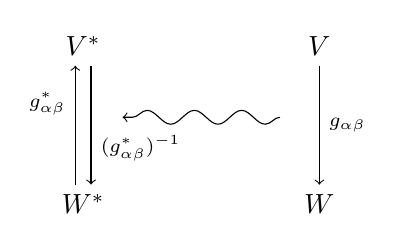
\begin{tikzpicture}
	\node (1) at (-1.5,1) {$V^*$}; \node (2) at (1.5,1) {$V$}; \node (3) at (-1.5,-1) {$W^*$}; \node (4) at (1.5,-1) {$W$};
	\draw[->] (2) --node[right,font=\scriptsize] {$g_{\alpha\beta}$} (4);
	\draw[->,transform canvas={xshift=1mm}] (1) --node[anchor=north west,font=\scriptsize] {$(g^*_{\alpha\beta})^{-1}$} (3);
	\draw[->,transform canvas={xshift=-1mm}] (3) --node[anchor=south east,font=\scriptsize] {$g_{\alpha\beta}^*$} (1);
	\draw[->,transform canvas={yshift=1mm},decorate,decoration={snake,segment length=6mm}] (1,0) -- (-1,0);
\end{tikzpicture}\end{center}

\begin{Dfn}
Es sei $E \xrightarrow{\pi} M$ ein Vektorb"undel "uber M. Ein \CmMark{Schnitt} in $E$ ist eine glatte Abbildung $S: M \to E$ mit $\pi \circ S = \Id_M$, also $S(p) \in E_p = \pi^{-1}(p)$. Der Raum der Schnitte wird mit $\Gamma(E)$ bezeichnet. $\Gamma(E)$ ist ein $C^{\infty}$-Modul.
\end{Dfn}


%%%
%%% 10. Vorlesung <2012-11-16 Fri>
%%% 

\textcolor{red}{Abbildung 10.1 Schnitt}

\textcolor{red}{Abbildung 10.2 Diagramm Schnitt}

Die $S_i$ bilden punktweise eine Basis der Fasern.

Die Schnitte des $(r,s)$-Tensorbündels $\Gamma(\T_s^r(\T M)) = \mathcal T_s^r(M)$ bezeichnet man als \CmMark{$(r,s)$-Tensorfelder} auf $M$. Die $(1,0)$-Tensorfelder sind genau die Vektorfelder auf $M$; $\mathcal T_0^1(M) = \mathcal V(M)$. Es bezeichne $\mathcal V^{*}(M) = \mathcal T_1^0(M)$ den Raum der $(0,1)$-Tensorfelder.

\begin{Prop}
Die $(r,s)$-Tensorfelder auf $M$ entsprechen genau den $C^{\infty}(M)$-multilinearen Abbildungen
	\[ \underbrace{\mathcal V^{*}(M) \X \cdots \X \mathcal V^{*}(M)}_{r-\text{mal}} \X \underbrace{\mathcal V(M) \X \cdots \X \mathcal V(M)}_{s-\text{mal}} \to C^{\infty}(M) \]
verm"oge der linearen Forsetzung
\begin{align*}
	p \mapsto & X_1 \otimes \cdots \otimes X_r \otimes \omega_1 \otimes \cdots \otimes \omega_s (\eta_1, \ldots, \eta_r, Y_1, \ldots, Y_s)\\
	& = \eta_1(X_1)\eta_2(X_2)\cdots\eta_r(X_r) \cdot \omega(Y_1)\cdots \omega_s(Y_s) (p)
\end{align*}
\end{Prop}

Der Beweis sei als Übung überlassen.

\begin{bsp}\begin{enumerate}[label=\arabic*)]
\item
	Ist $f \in C^{\infty}(M)$, so ist durch sein Differential
	\begin{align*}
		\dop f|_p(X_p) \textcolor{red}{=} X_p(f)
	\end{align*}
	ein $(0,1)$-Tensorfeld gegeben.
\item
	Die Lieklammer $[\cdot,\cdot]$ ist \emph{nicht} $C^{\infty}(M)$-linear, also kein Tensorfeld.
\end{enumerate}\end{bsp}

Ein Element von $\T_p^*M$ bezeichnet man als \CmMark[Kotangentialvektor]{Kotangentialvektoren}, $\T_p^*M$ als \CmMark{Kotangentialvektorraum} und das Bündel $\T^{*}M$ als \CmMark{Kotangentialbündel}. \textcolor{red}{(in der Vorlesung wurde das Element von $\T_p^*M$ selbst das Kotangententialvektorraum bezeichnet und der kotangentialvektor wurde "uberhaupt nicht er"ahnt, das erscheint falsch, also haben wir es ge"andert)}

Ist $(\varphi, U)$ eine Karte von $M$, dann bilden die Differentiale $\dop \varphi^i = \dop x^i$ der Koordinatenfunktionen (punktweise) eine Basis von $\T_p^{*}M$, denn
\begin{align*}
  \dop x^i|_p\left(\pdifffrac[p]{}{x^i}\right) = \pdifffrac{}{x^j}(\varphi^i) = \delta_j^i.
\end{align*}
Die $\dop x^i$ sind also \textcolor{red}{paarweise} linear unabhängige $(0,1)$-Tensorfelder über dem Kartengebiet $U$.

Ist $\psi$ eine weitere Karte und bezeichnen $\pdifffrac{}{y^i}$ beziehungsweise $\dop y^i$ die entsprechenden Koordinaten(ko)tangentialvektoren, so gilt:
	\[ \dop x^i = \sum \alpha_j^i\dop y^j \]
mit
	\[ \alpha_j^i \overset{!}{=} \dop x^i\left(\pdifffrac{}{y^j}\right) = \sum \alpha_k^i \underbrace{\dop y^k\left(\pdifffrac{}{y^j}\right)}_{\delta_j^k} \]
denn
	\[ \alpha_j^i = \textcolor{red}{\pdifffrac{}{y^j}(\varphi^i)} = \pdifffrac{p^i}{y^i} = \partial_j(\varphi^i\circ \psi^{-1}) \]
Es gilt also $\alpha = \D(\psi \circ \varphi^{-1})^{x^{-1}}$, vergleiche Satz 2.10 \textcolor{red}{(richtige Nummer hier, Nummerierung in Kapitel 2 korrigieren)}
\begin{align*}
  \pdifffrac{}{x^i} = \sum \partial_i (\psi^j \circ \varphi^{-1})\pdifffrac{}{y^j}.
\end{align*}
Diese transponierten Inversen der Differentiale der Kartenwechsel sind geanu die Übergangsfunktionen $h_{\alpha\beta} = (g_{\alpha\beta}^{*})^{-1}$ in der Definition von $(\T M)^{*} = \T^{*}M$.

Ist $S$ ein Tensorfeld vom Typ $(0,s)$ auf einer Mannigfaltigkeit $N$ und $\Phi \colon M \to N$ eine glatte Abbildung.
\begin{center}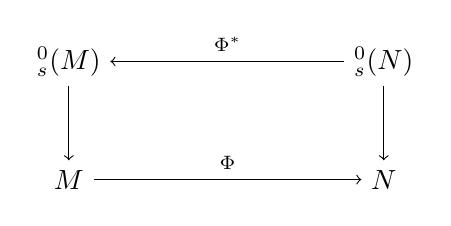
\begin{tikzpicture}
	\node (1) at (-2,0.75) {$\calT_s^0(M)$};
	\node (2) at (2,0.75) {$\calT_s^0(N)$};
	\node (3) at (-2,-0.75) {$M$};
	\node (4) at (2,-0.75) {$N$};
	
	\draw[->] (2) --node[above,font=\scriptsize]{$\Phi^*$} (1);
	\draw[->] (1) -- (3);
	\draw[->] (2) -- (4);
	\draw[->] (3) --node[above,font=\scriptsize]{$\Phi$} (4);
\end{tikzpicture}\end{center}
	\[ \begin{array}{rccc} S \colon & \mathcal V(N) \X \cdots \X \mathcal V(N) &\to& C^{\infty}(N)\\
		\Phi^{*}S \colon & \mathcal V(M) \X \cdots \X \mathcal V(M) &\to& C^{\infty}(M) \end{array} \]
Dann ergibt
	\[ \Phi^{*}S(X_{1},\ldots,X_{s}) = S(\Phi_{*}X_{1},\ldots,\Phi_{*}X_{s}) \]
ein $(0,s)$-Tensorfeld auf $M$, das entlang $\Phi$ zurückgezogene Tensorfeld (\CmMark{pullback}).

Es gilt $\Phi^{*}(S \otimes T) = \Phi^{*}S \otimes \Phi^{*}T$ für $S \in \mathcal T_s^0(N), T \in \mathcal T_t^0(N)$.
Ist $\Psi \colon P \to M$ glatt, so gilt
	\[ (\Phi \circ \Psi)^{*} = \Psi^{*} \circ \Phi^{*}.\]

Ist $\Phi$ ein Diffeomorphismus, so lässt sich $\Phi^{*}$ für beliebige Tensorfelder $S \in \mathcal T_s^r(M)$ definieren:
	\[ \begin{array}{rl} p \mapsto& \Phi^{*}S (\omega_1,\ldots,\omega_r,X_1,\ldots,X_s)(p)\\
		& S((\Phi^{*})^{-1}\omega_1, \ldots, (\Phi^{*})^{-1}\omega_{r}, \Phi_{*}X_1,\ldots,\Phi_{*}X_s)(p) \end{array} \]
mit
	\[ \begin{array}{rccc} S \colon& \underbrace{\mathcal V^{*}(N) \cdots \mathcal V^{*}(N)}_{r\text{-mal}} \X \underbrace{ \mathcal V(N) \cdots\mathcal V(N)}_{s\text{-mal}} &\to& C^{\infty}(N)\\
		\Phi^*S \colon& \mathcal V^{*}(M) \cdots \mathcal V^{*}(M) \X \mathcal V(N) \cdots\mathcal V(N) &\to& C^{\infty}(M) \end{array} \]
	\[ \begin{array}{rccc} \textcolor{red}{\omega \in}& \mathcal V^{*}(M) = \mathcal T_1^0(M) &\to& C^{\infty}(M)\\
		\textcolor{red}{X \in}& \mathcal V(M) = \calT_0^1(M) &\to& C^{\infty}(M) \end{array} \]
Insbesondere: $X \in \mathcal T_0^1(M) = \mathcal V(M) = \{\calV^*(M) \to C^{\infty}(M)\}$
\begin{align*}
  \Phi^{*}X(\omega) = X((\Phi^{*})^{-1}\omega) = ((\Phi^{*})^{-1}\omega)(X) = \omega(\Phi_{*}^{-1}X)
\end{align*}
also $\Phi^{*}X = \Phi_{*}^{-1}X$.

\begin{bsp}[Anwendung]
  Es sei $(\varphi_{\alpha},U_{\alpha})$ ein Atlas von $M$. Dann ist jedes $\varphi_{\alpha}$ ein Diffeomorphismus von $U_{\alpha}$ auf $\varphi_{\alpha}(U_{\alpha}) = V_{\alpha} \subset \R^m$. Ist $S \in \mathcal T_s^r(M)$, so ist
  \begin{align*}
    S_{\alpha} = (\varphi_{\alpha}^{-1})^{*}S|_{U_\alpha}
  \end{align*}
  ein $(r,s)$-Tensorfeld auf $V_{\alpha}$.

  \textcolor{red}{Abbildung 10.4 Diagram Beispiel/Anwendung}

  Für alle $\alpha, \beta$ mit $U_{\alpha} \cap U_{\beta}$ gilt
  \begin{align*}
    (\varphi_{\alpha} \circ \varphi_{\beta}^{-1})^{*}S_{\alpha}|_{V_{\alpha} \cap V_{\beta}} & = (\varphi_{\alpha} \circ \varphi_{\beta}^{-1})^{*}\left((\varphi_{\alpha}^{-1})^{*}S|_{U_{\alpha}}\right)|_{V_{\alpha}\cap V_{\beta}}\\
    & = \left.(\varphi_{\beta}^{-1})^{*} \circ \varphi_{\alpha}^{*} \circ (\varphi_{\alpha}^{-1})^{*} S|_{U_{\alpha}}\right|_{V_{\alpha} \cap V_{\beta}}\\
    & = \left.(\varphi_{\beta}^{-1})^{*}S|_{U_{\beta}}\right|_{V_{\alpha} \cap V_{\beta}}\\
    & = S_{\beta}|_{V_{\alpha} \cap V_{\beta}}
  \end{align*}
  Ist umgekehrt $S_\alpha$ eine Familie von $(r,s)$-Tensorfeldern auf $V_{\alpha}$ mit obigem Transformationsverhalten, so definiert dies ein $(r,s)$-Tensorfeld auf $M$.
\end{bsp}

\begin{Dfn}
  Es sei $X \in \mathcal V(M)$ mit dem Fluss $\gamma$ und $S \in \mathcal T_s^r(M)$ ein glattes Vektorfeld auf $M$. Dann heißt
  \begin{align*}
    \mathcal L_X S = \difffrac[t=0]{}{t}(\gamma^{t*}S)
  \end{align*}
  die \CmMark{Lieableitung} von $S$ in Richtung $X$.
\end{Dfn}

\begin{emptythm}[Eigenschaften]\begin{enumerate}[label=\arabic*)]
\item
	$f \in \mathcal T_0^0(M) = C^{\infty}(M)$. Dann ist $\mathcal L_Xf = \dop f (X) = X(f)$.
\item
	$X,Y \in \mathcal T_0^1(M) = \mathcal V(M)$, so gilt
	\begin{align*}
		\mathcal L_XY = [X,Y].
	\end{align*}
\item
	Für $S \in \mathcal T_s^r(M), T \in \mathcal T_{s'}^{r'}(M)$ gilt:
	\begin{align*}
		\mathcal L_X(S \otimes T) = (\mathcal L_XS) \otimes T + S \otimes (\mathcal L_X T).
	\end{align*}
\end{enumerate}\end{emptythm}


\section{Differentialformen und die äußere Ableitung}

\begin{Dfn}
  Das Vektorbündel $\Lambda^k(\T^{*}M)$ wird mit $\Lambda^k(M)$ bezeichnet und der Raum seiner Schnitte $\Gamma(\Lambda^k(\T^{*}M))$ mit $\Omega^k(M)$. Die Elemente von $\Omega^k(M)$ heißen \CmMark{Differentialformen} vom Grad $k$ oder kurz \CmMark{$k$-Formen} auf $M$.
\end{Dfn}

Ist $(\varphi, U)$ eine Karte von $M$, so bilden die Differentiale der Koordinatenfunktionen $\dop x^i = \dop \varphi^i$ eine Basis von $\T^{*}M$.
Diese sind (lokale) Schnitte in $\Lambda^1(\T^{*}M)$, also lokal $1$-Formen. Das Differential von $f \in C^{\infty}(M)$ ist eine $1$-Form $\dop f(X) = X(f)$.
Lokal gilt $\dop f = \sum f_i \dop x^i$, wobei $f_i = \dop f \left(\pdifffrac{}{x^i}\right) = \pdifffrac{}{x^i}(f) = \pdifffrac{f}{x^i}$.

Desweiteren sind (lokal) die $\left( \begin{smallmatrix} m \\ k\end{smallmatrix} \right)$ $k$-Formen $\dop x^{i_1} \wedge \ldots \wedge \dop x^{i_k}$ mit $i_1 < \cdots < i_k$ eine Basis von $\Omega^k$. Jede $k$-Form $\omega$ ist lokal von der Gestalt
\begin{align*}
  \omega = \sum_{\mathclap{i_1 < \cdots < i_k}}f_{i_1,\ldots,i_k}\dop x^{i_1} \wedge \cdots \wedge \dop x^{i_k}.
\end{align*}


%%% Local Variables: 
%%% mode: latex
%%% TeX-master: "../skript-diffgeom"
%%% End: 
